\chapter{Foundations}
\label{sec:foundations}

This chapter will show and explain the foundations necessary for this work. The term \textbf{Domain Adaptation} aswell as what \textbf{synthetic} and \textbf{real} means in the context of this work, will be defined and some examples shown. Furthermore the relevant \textbf{Neural Network} architectures will be shown and explained. Specifically \textbf{Convolutional Neural Networks} and \textbf{Generative Adversarial Networks}.


\section{Domain Adaptation}
As described in \cite{DBLP:journals/corr/Csurka17},
Domain Adaptation is the task of transfering a machine learning model that is working well on a source data distribution to a related target data distribution. In this work we will focus on the adaptation from synthetic to real images. When talking about a synthetic image we are implying it was rendered from a virtual scene through a rendering engine like for example blender's ''Cycles`` \cite{Cycles} or graphics engine like Unity \cite{Unity}. We define real images as taken from a real-world scene through some kind of camera. See Figure \ref{fig:DA_examples} for an example of synthetic and real images. Other examples of domains are an image of a painting in the style of a particular artist, images of an object from different viewpoints, and many more. 

\begin{figure}
	\centering
	 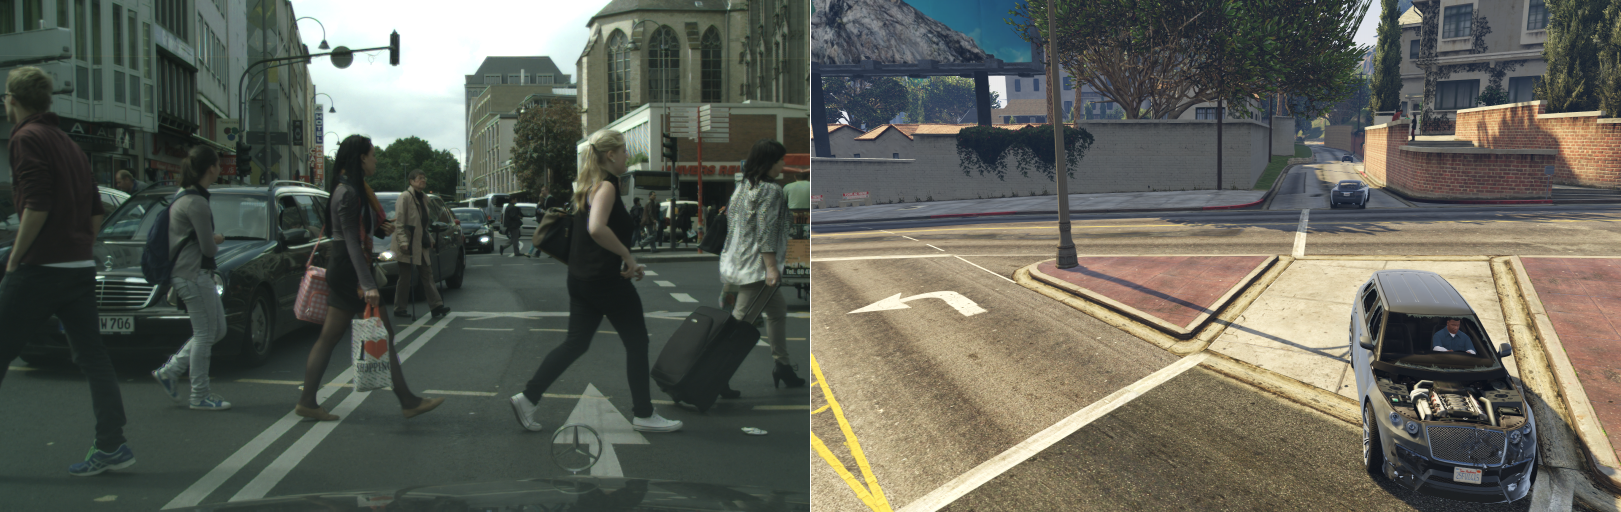
\includegraphics[width=0.8\textwidth]{../images/DA_examples_cityscapes_gta.png}
	\caption{Example images for the the two domains relevant for this work. A real image from the cityscapes dataset \cite{Cordts_2016_CVPR} (left) and a synthetic image from the GTA5 dataset \cite{Richter_2016_ECCV} (right)}
	\label{fig:DA_examples}
\end{figure}

\section{Semantic Segmentation}
Semantic Segmentation is one of the most important aspects in autonomous driving. It is the task of semantically segmentating objects in an image, i.e. labeling each pixel according to what object it belongs to. See Figure \ref{fig:semseg} for examples.

\begin{figure}
	\centering
	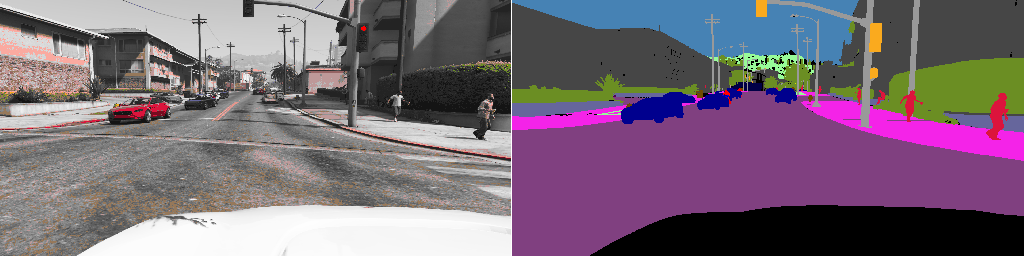
\includegraphics[width=\textwidth]{../images/semseg.png}
	\caption{Examples of a semantic segmentation images. Image taken from the GTA5 dataset \cite{Richter_2016_ECCV} (left) and same image mapped to Cityscapes Id values (pixel values 0-19, adapted to brighter values here to improve visibility). Streets in purple, sidewalks in pink, pedestrians red, cars, blue in the left image, which is mainly for visualization purposes. The right image is used for processing.}
	\label{fig:semseg}
\end{figure}



\section{Generative Adversarial Networks}
Generative Adversarial Networks (GANs) implement a two-player-game:\\
A Discriminator learns from a given data distribution what is ``real''. The Generator generates data. The goal of the generator is to fool the discriminator into believing the generated data is ``real'' i.e. tries to create samples coming from the same distribution as the ``real'' data. The discriminator will label anything as ``fake'' that doesn't resemble the learned ``real'' data distribution. This can be described as a 2 classes classification, with classes real and fake). This way GANs can learn to generate realistically looking images of faces, translate images of art from one style to another and improve semantic segmentation.
The generative model generally uses \textit{maximum likelihood estimation}. In \cite{DBLP:journals/corr/Goodfellow17} it is described in the following way:
\begin{quote}
	The basic idea of maximum likelihood is to define a model that provides an estimate of probability distribituion, parametereized by parameters $\theta$. We then refer to the \textbf{likelihood} as the probability that the model assigns to the training data: $\prod_{i=1}^{m}p_{\text{model}}(x^{(i)}; \theta)$
\end{quote}
The parameter $\theta$ that maximizes the likelihood of the data is better found in $\log$ space
\begin{align}
	\theta^* &= \underset{\theta}{\arg \max} \prod_{i = 1}^{m} p_{\text{model}} (x^{(i)}; \theta)\\
	&= \underset{\theta}{\arg \max} \log \prod_{i=1}^{m} p_{\text{model}}(x^{(i)}; \theta)\\
	&= \underset{\theta}{\arg \max} \sum_{i = 1}^{m} \log p_{\text{model}}(x^{(i)}; \theta)
\end{align}
as the maximum of the function is at the same $\theta$ value and we now have a sum which aswell eliminates the possibility of having underflow by multiplying multiple very small probabilities together.
Formally GANs are a structured probabilistic model (more info: Chapter 16 of Goodfellow et al. 2016) containing latent variables z and observed variables x.
The generator is defined by a function G that takes $\mathbf{z}$ as input and uses $\theta^{(G)}$ as parameters, the discriminator by a function D that takes $\mathbf{x}$ as input and uses $\theta^{(D)}$ as parameters. Both players have cost functions that are defined in terms of both players' parameters. The discriminator  wishes to minimize $J^{(D)}(\theta^{(D)}, \theta^{(G)})$ and must do so by controlling only $\theta^{(D)}$. This is analogous for the generator: he tries to minimize $J^{(G)}(\theta^{(D)}, \theta^{(G)})$ while controlling only $\theta^{(G)}$. In contrast to an optimization problem that has a solution that is the (local) minimum (a point in parameter space where all neighboring points have greater or equal cost), the GAN objective is a game. The solution to a game is a Nash equilibrium \cite{Nash48}, meaning that each player chooses the best possible option or strategy in respect to what the other player(s) choose. Here the Nash equilibrium is a tuple $(\theta^{(D)}, \theta^{(G)})$ that is a local minimum of $J^{(D)}$ with respect to $\theta^{(D)}$ and a local minimum $J^{(G)}$ with respect to $\theta^{(G)}$.
\textbf{The generator} is simply a differentiable function G. When $\mathbf{z}$ is sampled from some simple prior distribution, G(z) yields a sample of $\mathbf{x}$ drawn from $p_{\text{model}}$. Typically a deep neural network is used to represent G. \\
The game plays out in two scenarios. The first is where the discriminator D is given random training examples $\mathbf{x}$ from the training set. The goal of the discriminator here is for $D(\mathbf{x})$ to be near 1. In the second scenario, random noise $\mathbf{z}$ is input to the generator. The discriminator then receives input $G(\mathbf{z})$, a fake sample by the generator. The discriminator strives to make $D(G(\mathbf{z}))$ approach 0 while the generator tries to make that approach 1. The games Nash equilibrium corresponds to $G(\mathbf{z})$ being drawn from the same distribution as the training data. Under the assumption that the inputs to the discriminator are half real and half fake, this corresponds to $D(\mathbf{x}) = \frac{1}{2}$ for all $\mathbf{x}$.

\paragraph{Training}
On each step, two minibatches are sampled: a minibatch of $\mathbf{x}$ values from the dataset and one of random noise $\mathbf{z}$. Then two gradient steps are made simultaneously (simultaneous SGD): one updating $\theta^{(D)}$ to reduce $J^{(D)}$ and one updating $\theta^{(G)}$ to reduce $J^{(G)}$.

\paragraph{Cost functions} There are many different cost functions that can be used for GANs. See chapter \ref{sec:techniques} for the ones that the techniques in this work use.


\subsection{Disadvantages}
\paragraph{non-convergence} When training GANs, while updating one player so that he makes the best possible current move and goes downhill the loss curve it is possible that the counterfeit player gets updated into going uphill the loss curve. This is in contrast to optimization problems where one tries to find a (local) minimum of the loss curve for example through stochastic gradient decent (SGD). Because there is only one gradient instead of the two in GAN objectives, the model generally makes reliable downhill progress during training. The result is that GANs often oscillate in practice due to the nature of having two players playing against each other, each trying to achieve the optimal outcome for themselves.

\paragraph{mode collapse} occurs when the generator learns to map different inputs to the same output. This results in generated data that is missing diversity. A solution is proposed in \cite{DBLP:journals/corr/ZhuPIE17}: Using a batch history of 50 images so that the discriminator also learns the distribution of images of the training data and can therefore make sure that the generator will not generate the same small set of images. Partial mode collapse refers to scenarios in which the generator makes multiple images containing the same color or texture themes, or multiple images containing different views of the same dog. See Figure \ref{fig:mode_collapse} for an example.

\begin{figure}
	\centering
	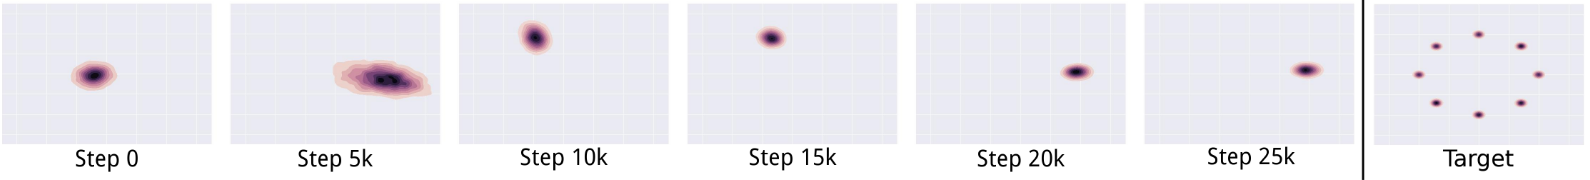
\includegraphics[width=\textwidth]{images/metz_et_al_mode_collapse.png}
	\caption{target data distribution of a toy dataset (right) and the data distribution of generated samples. Mind that the generated sample distribution hops from one mode to the next as the discriminator learns to recognize each mode as fake. Image from \cite{DBLP:journals/corr/MetzPPS16}}
	\label{fig:mode_collapse}
\end{figure}

\newpage

\subsection{Advantages} (From \cite{GAN_Projects})
\paragraph{unsupervised.} GANs are trained in an unsupervised manner. There is no ground truth (i.e. labeled data) or an external true or false feedback (reinforcement learning) necessary to train the network. This makes acquiring data cheaper and easier and therefore training GANs aswell. 

\paragraph{data generation.} GANs learn to generate data that is indistinguishable from real data. This is useful for many applications such as generating images that can be used by artists to quickly generate a few samples of an idea, generate text that can then be adjusted to a specific purpose, aswell as for audo and video.

\paragraph{learn density distribution.} GANs learn density distribution of data. In contrast to other models that can learn specific distributions, GANs can learn diverse, complex data distributions.

\paragraph{discriminator is a classifier.} The trained discriminator of GANs is a binary classifier and can be used as such. For example if the discriminator learns that images from real data contain a dog it can be used as to classify if an image contains a dog or not. 